%%%%%%%%%%%%%%%%%%%%%%%%
%\subsection{Navigating the PyETMG GUI}
%\label{sec:pyemtg_gui_navigation}
%%%%%%%%%%%%%%%%%%%%%%%%

\noindent Once in the PyEMTG \ac{GUI} a user is presented with a screen where they can use the File menu to either open an existing mission via an \ac{EMTG} options file or create a new mission. All PyEMTG GUI functionality can be accessed through a user's keyboard and mouse or soley using the keyboard. The ability to solely use a keyboard to interact with the PyEMTG GUI should also allow it to be compatible with assitive technology devices. The selections of the File menu contains keyboard shortcuts that a user can use for quick access to the File menu selections. 

\begin{figure}[H]
	\centering
	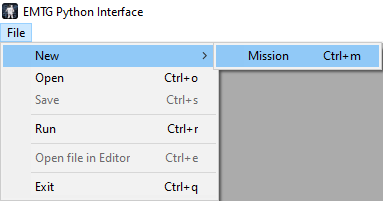
\includegraphics[width=0.7\linewidth]{../../shared_latex_inputs/images/pyemtg_file_new.png}
	\caption{EMTG File Menu}
\end{figure}
				
\noindent Once an EMTG mission is populated in the GUI, several tabs become visible to the user where they can alter values through several input fields (i.e. calanderCTRL pickers, text fields, check boxes, drop-down menus). 

\begin{figure}[H]
	\centering
	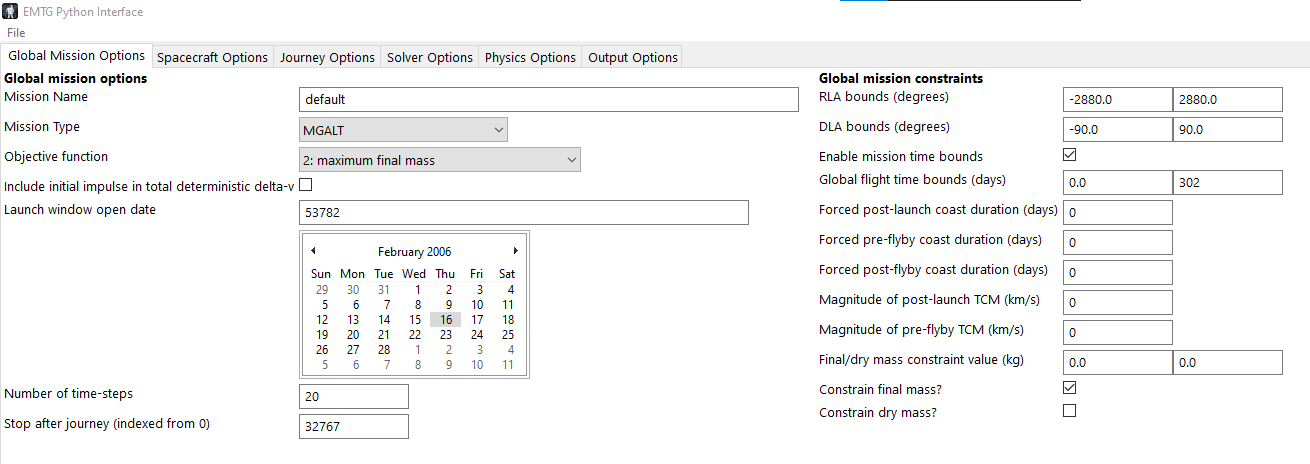
\includegraphics[width=0.7\linewidth]{../../shared_latex_inputs/images/pyemtg_global_options_tab.png}
	\caption{EMTG Global Mission Options Tab}
\end{figure}

\noindent The names of the tabs are as followed:
\begin{itemize}
	\item Global Mission Options
	\item Spacecraft Options
	\item Journey Options
	\item Solver Options
	\item Physics Options
	\item Output Options
\end{itemize}

\noindent The following are keyboard sequences that allow a user to navigate through the \ac{GUI} tabs:
\begin{itemize}
	\item Ctrl + Tab: Go to the next GUI Tab
	\item Ctrl + Shift + Tab: Go to the previous GUI Tab
	\item Shift + Tab: Go to a previous input field
	\item Tab: Go to the next input field
\end{itemize}

\noindent Once a user enters the calendarCTRL input field, the following keyboard sequences allow a user to select a date and navigate:
\begin{itemize}
	\item arrow keys: Move to a new day/Month/Year/Year-Range
	\item Tab: Exit calendar input field to next input field
	\item Shift+Tab: Exit calendar input field to previous input field
	\item Ctrl + up arrow: Zoom out upper calendar selection to be broader (e.g. going from month to year, year to year-range)
	\item Ctrl + down arrow: Zoom in upper calendar  selection to be narrower 
	\item Ctrl + left/right arrow: Move to next value of the upper calendar selection
\end{itemize}